\clearpage
\section{Řídící jednotka}
\indent\indent Tento modul slouží k ovládání celého rádia, nastavení a zobrazení přijímané frekvence a dále k řízení generátoru DDS pro ovládání výstupního kmitočtu lokálního oscilátoru.

Řídící jednotka je postavena na jednočipovém mikrokontroléru ATmega8, taktovaného na $11,0592~MHz$. Frekvence hodin není náhodná, ale je vybrána záměrně, jelikož díky této taktovací frekvenci může mikrokontrolér komunikovat s okolím pomocí rozhraní USART rychlostí $9600~Bdps$. K mikrokontroléru je připojen znakový LCD displej RC1602B2-BIW-CSX s řadičem HD44780. Jedná se o displej, který zobrazuje informaci ve dvou řádcích, každý po 16 znacích. Displej je použit k zobrazování frekvence přijímané stanice a velikosti ladícího kroku. Dále je k mikrokontroléru připojen rotační enkodér s vestavěným tlačítkem. Pro změnu frekvence nebo velikosti ladícího kroku. Na základě údajů získaných od operátora řídící jednotka nakonfiguruje DDS obvod v lokálním oscilátoru.


% vyvojak A
\begin{figure}[H]
	\centering
	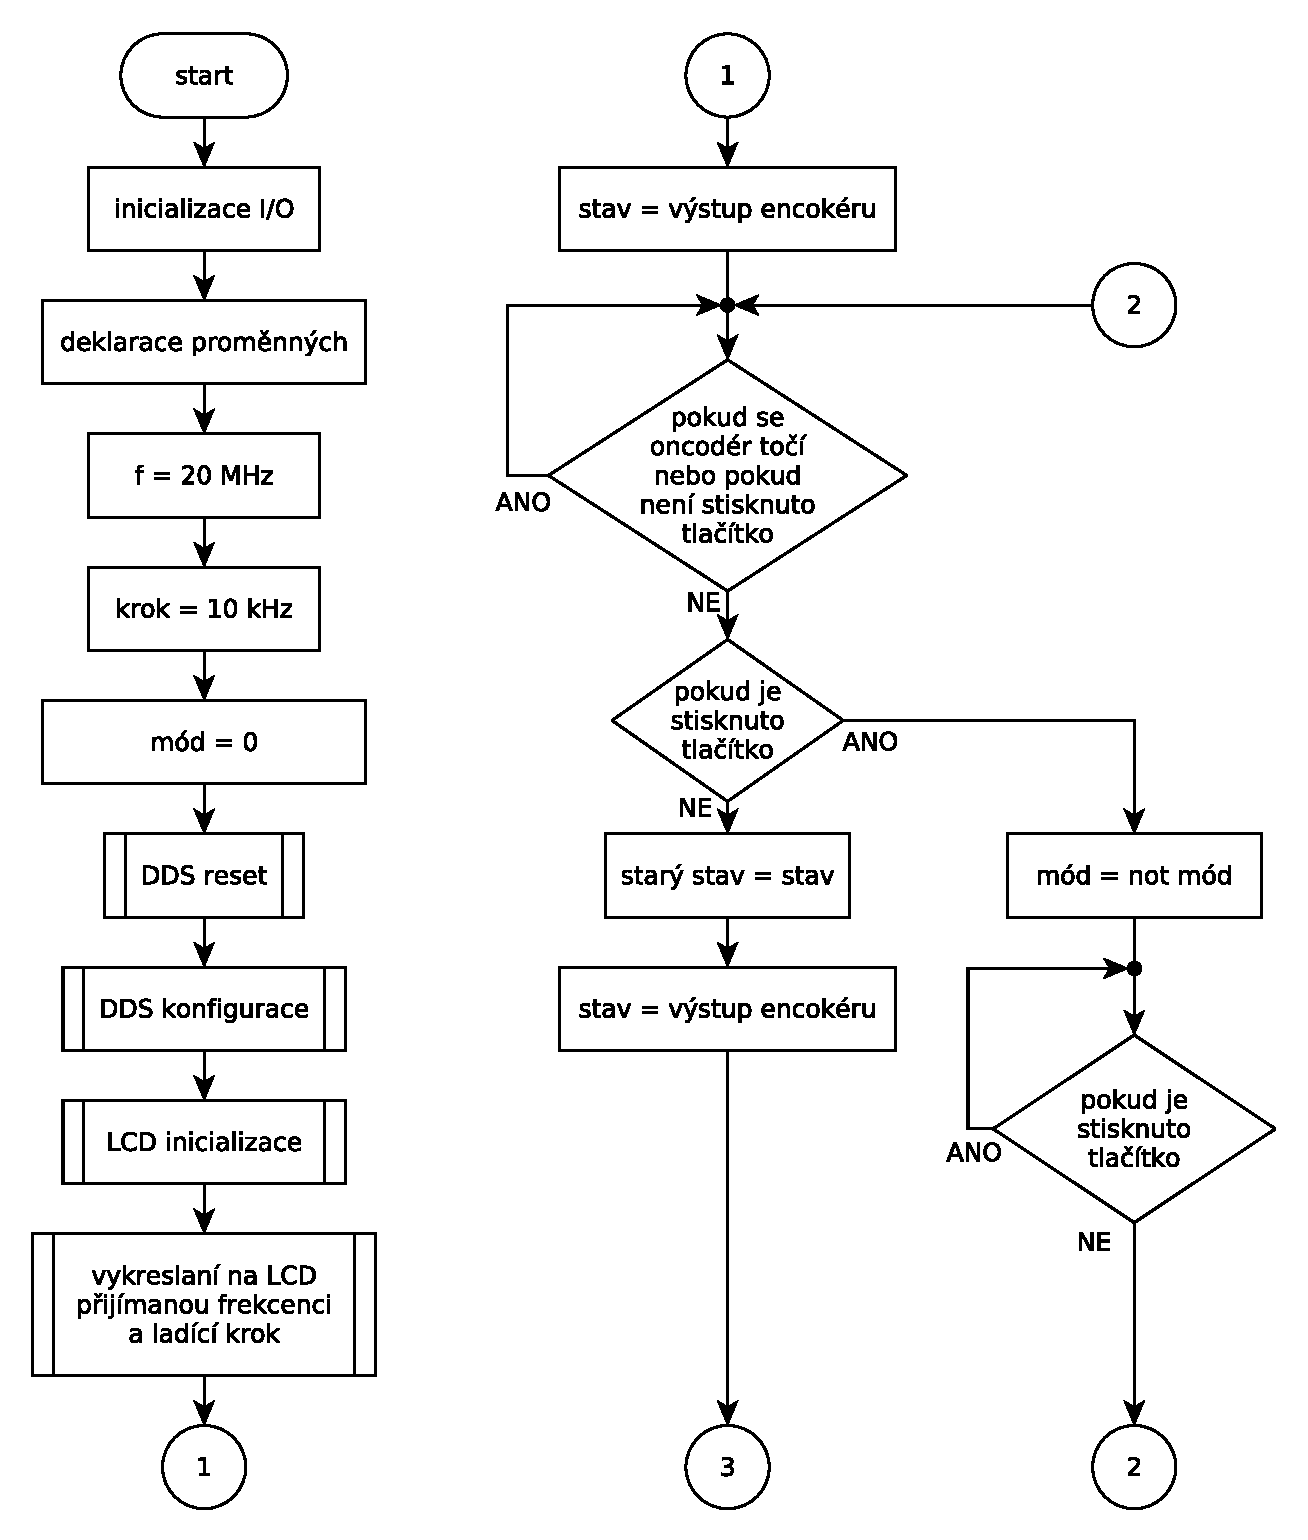
\includegraphics[height=150mm]{img/vyvojak_a.pdf}
	\caption{Vývojový diagram programu řídící jednotky část A}    		
\end{figure}

% vyvojak B
\begin{figure}[H]
	\centering
	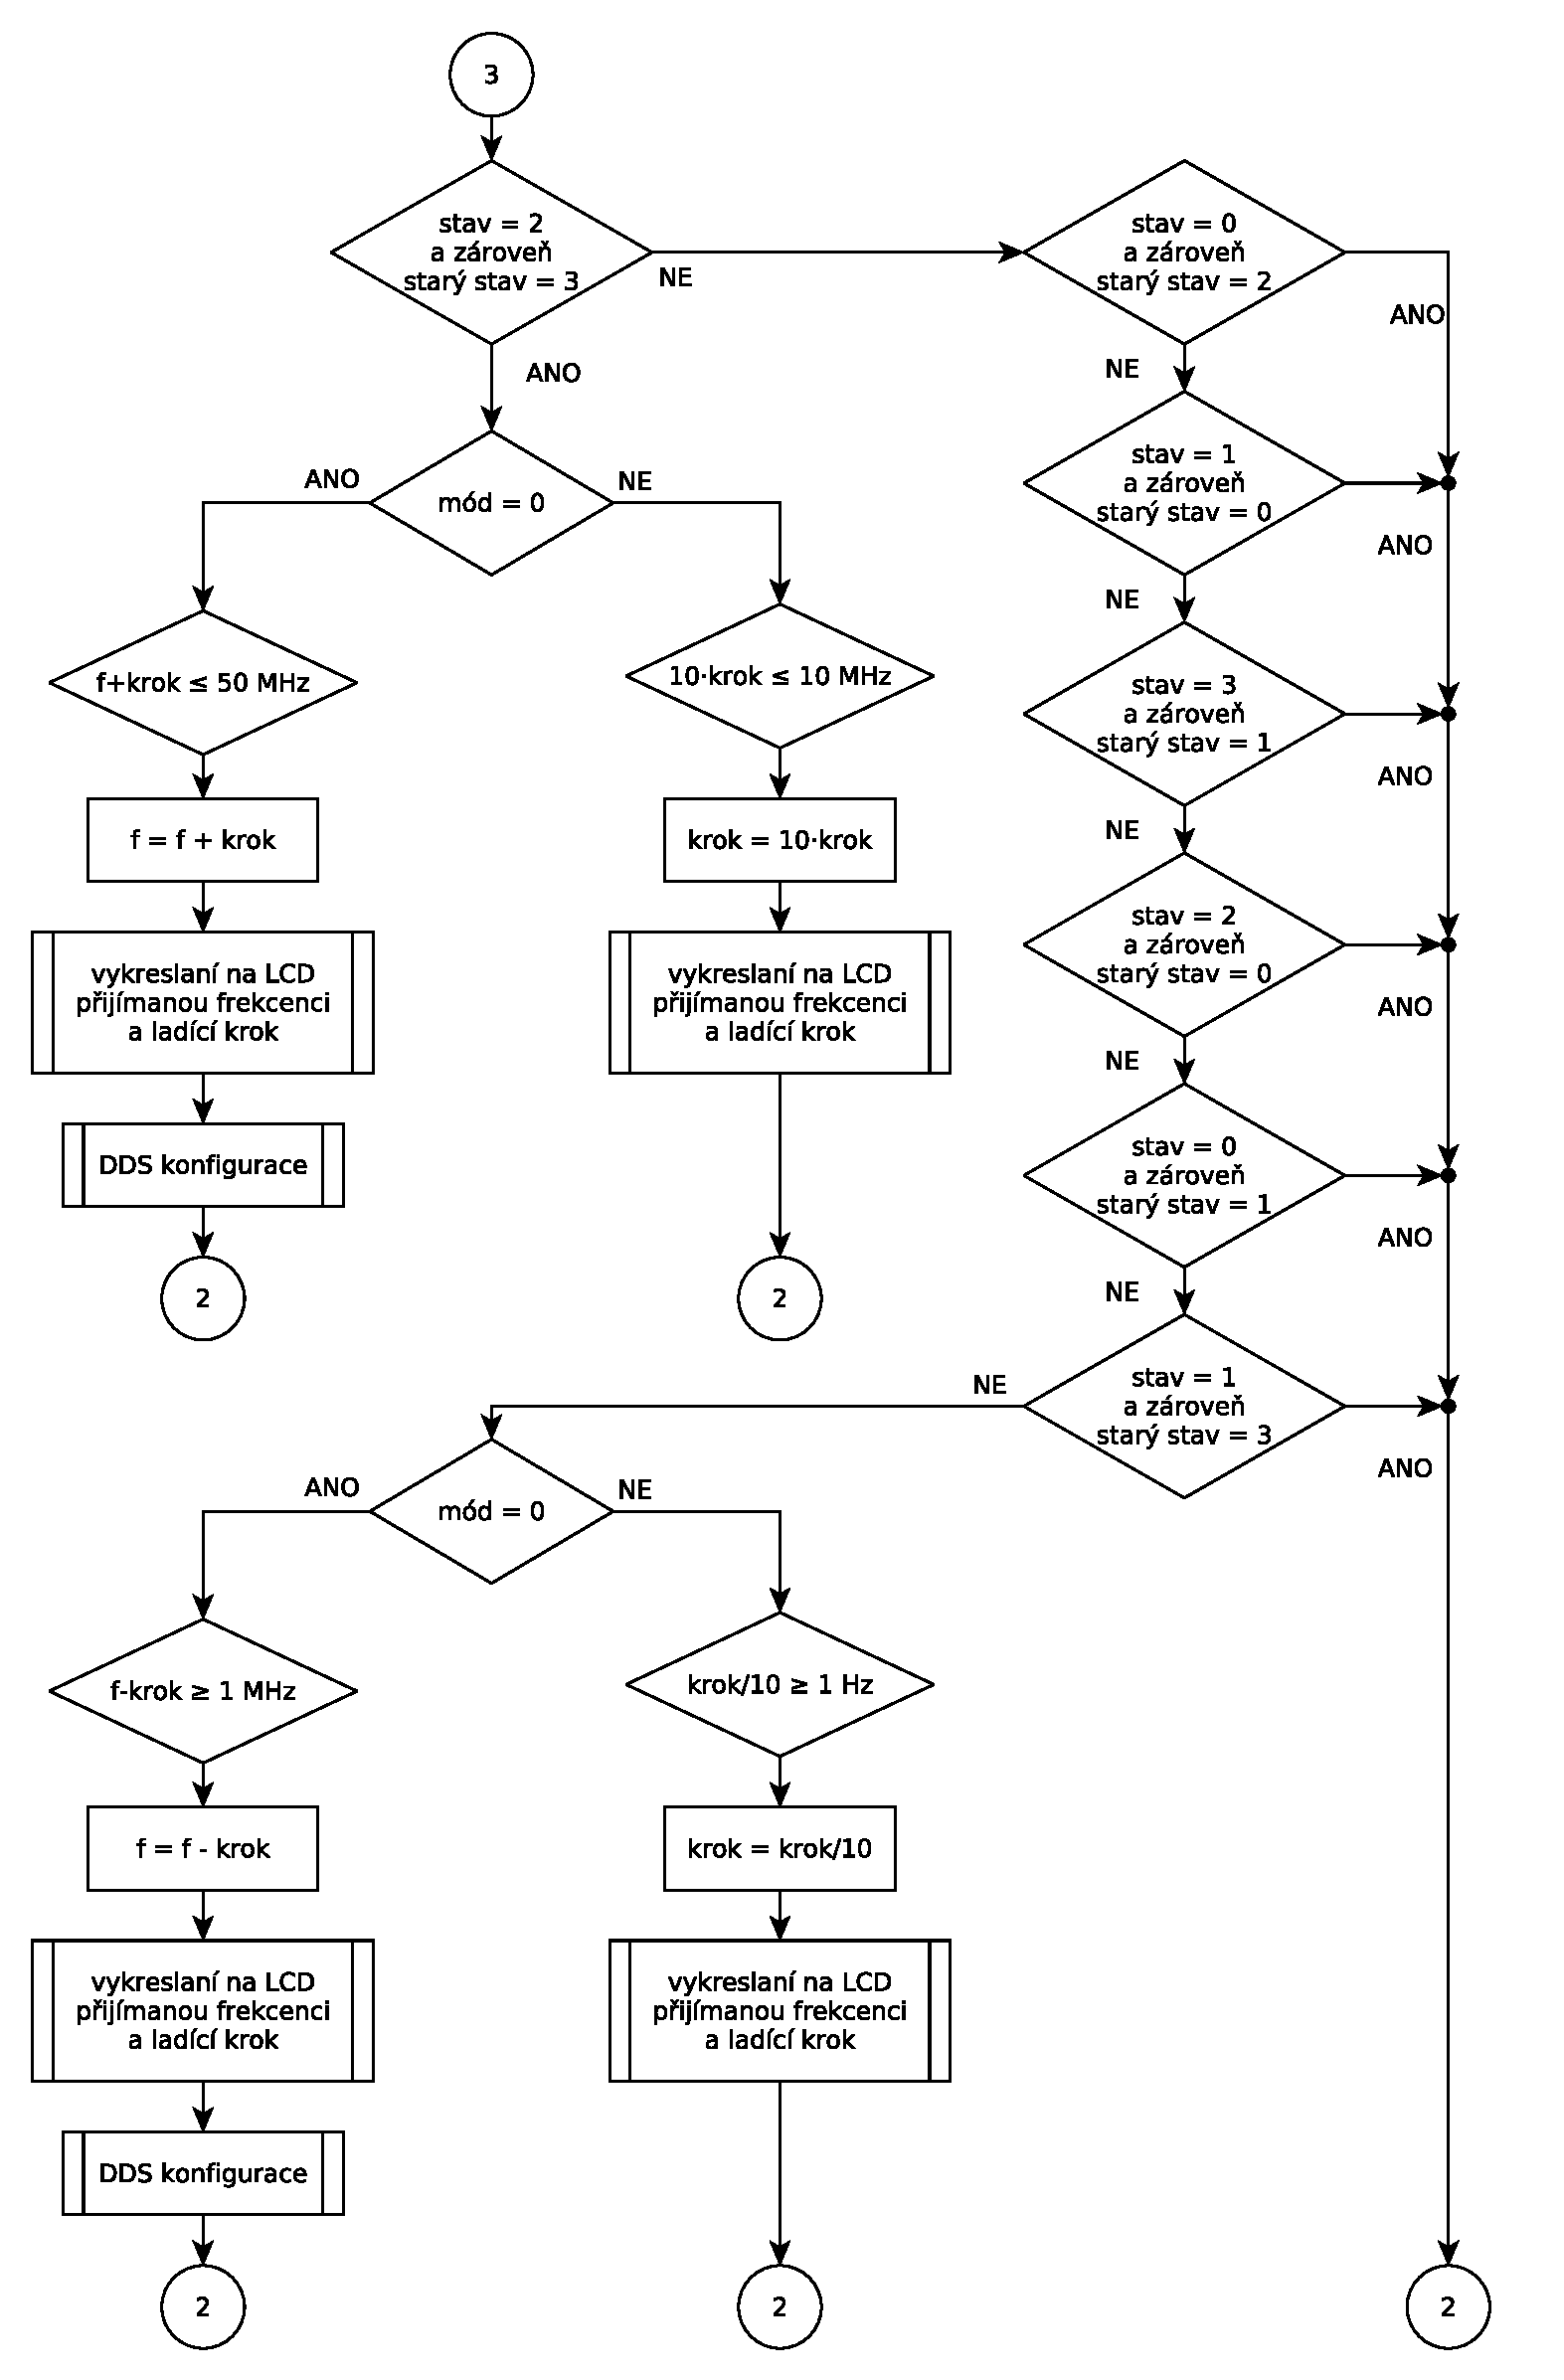
\includegraphics[height=220mm]{img/vyvojak_b.pdf}
	\caption{Vývojový diagram programu řídící jednotky část B}    		
\end{figure}


% schéma
\begin{landscape}
	\begin{figure}[h]
		\centering 	
		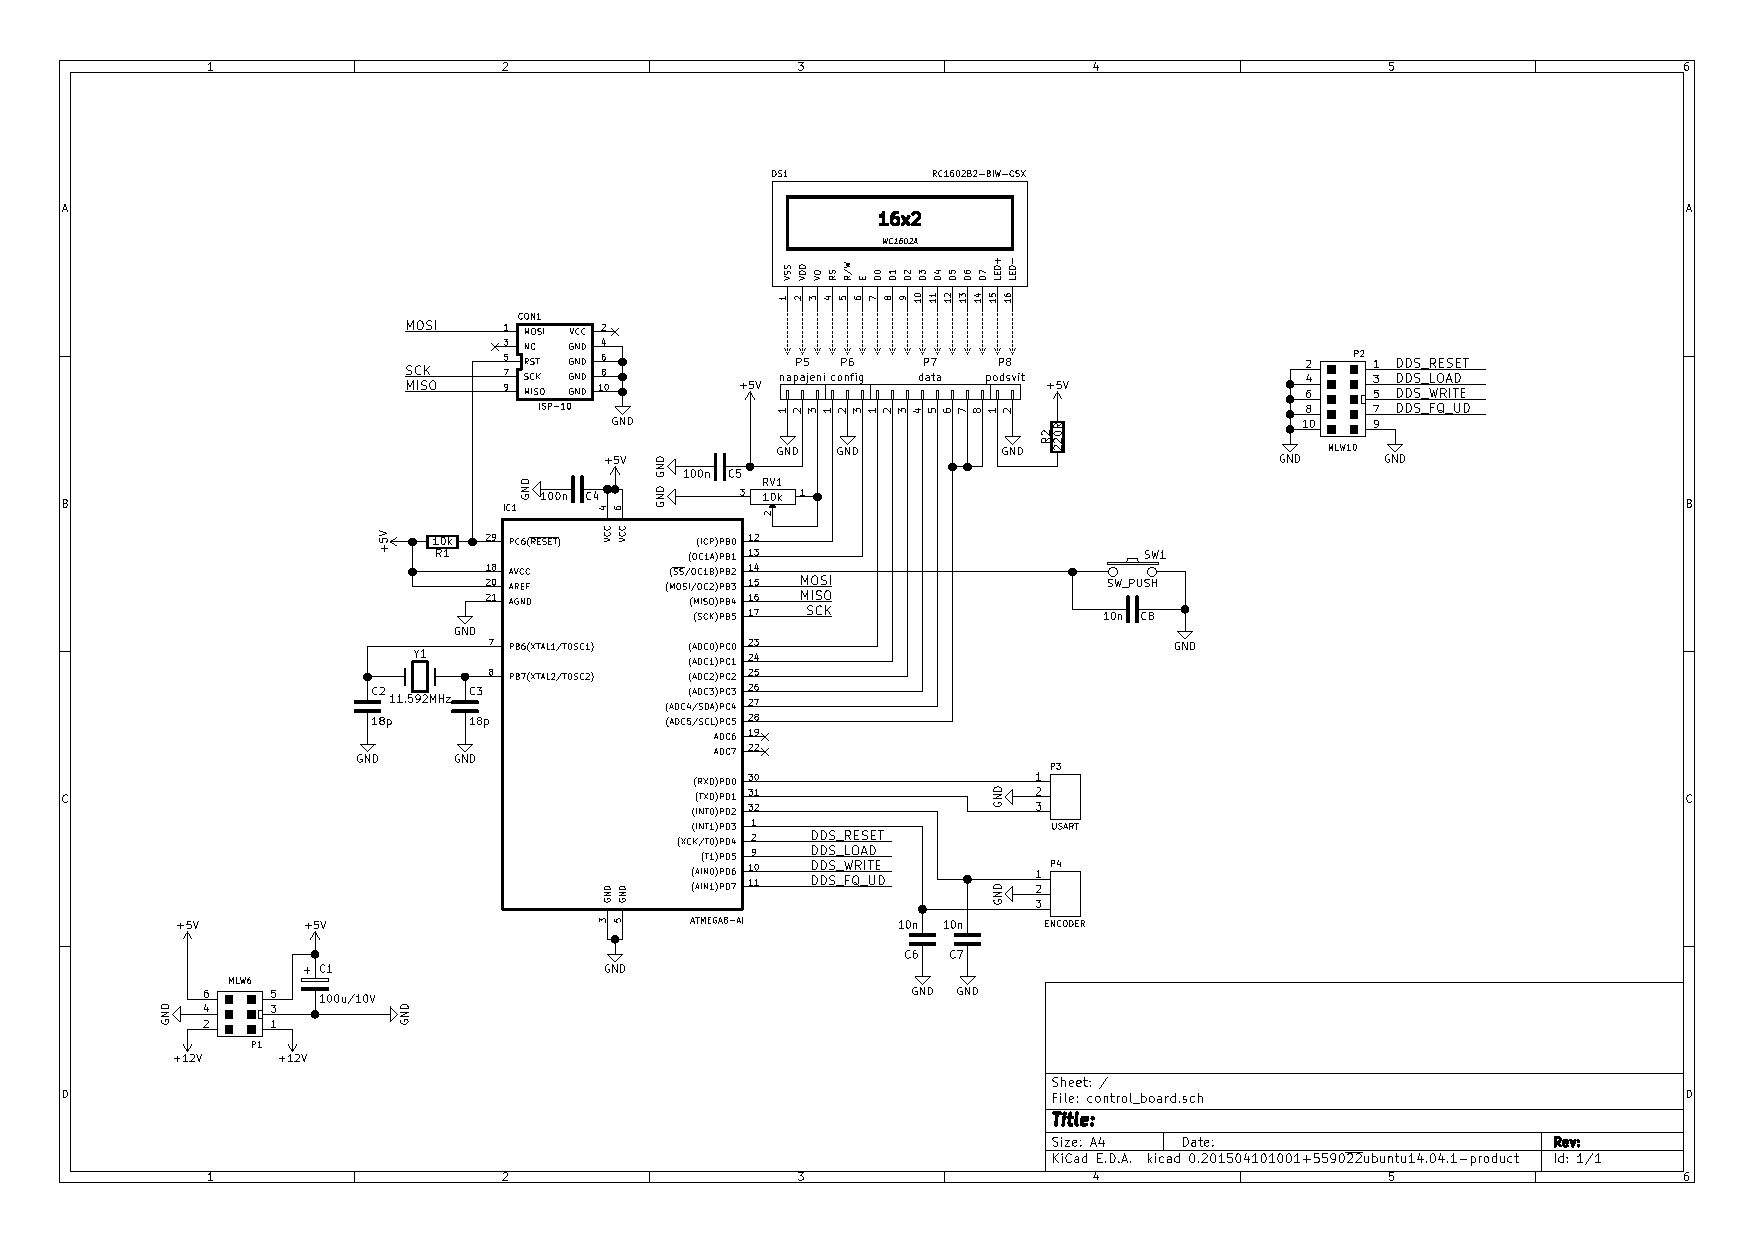
\includegraphics[height=\textwidth]{img/cu/sch.pdf}
		\caption{Schéma zapojení řídící jednotky}	
	\end{figure}
\end{landscape}
%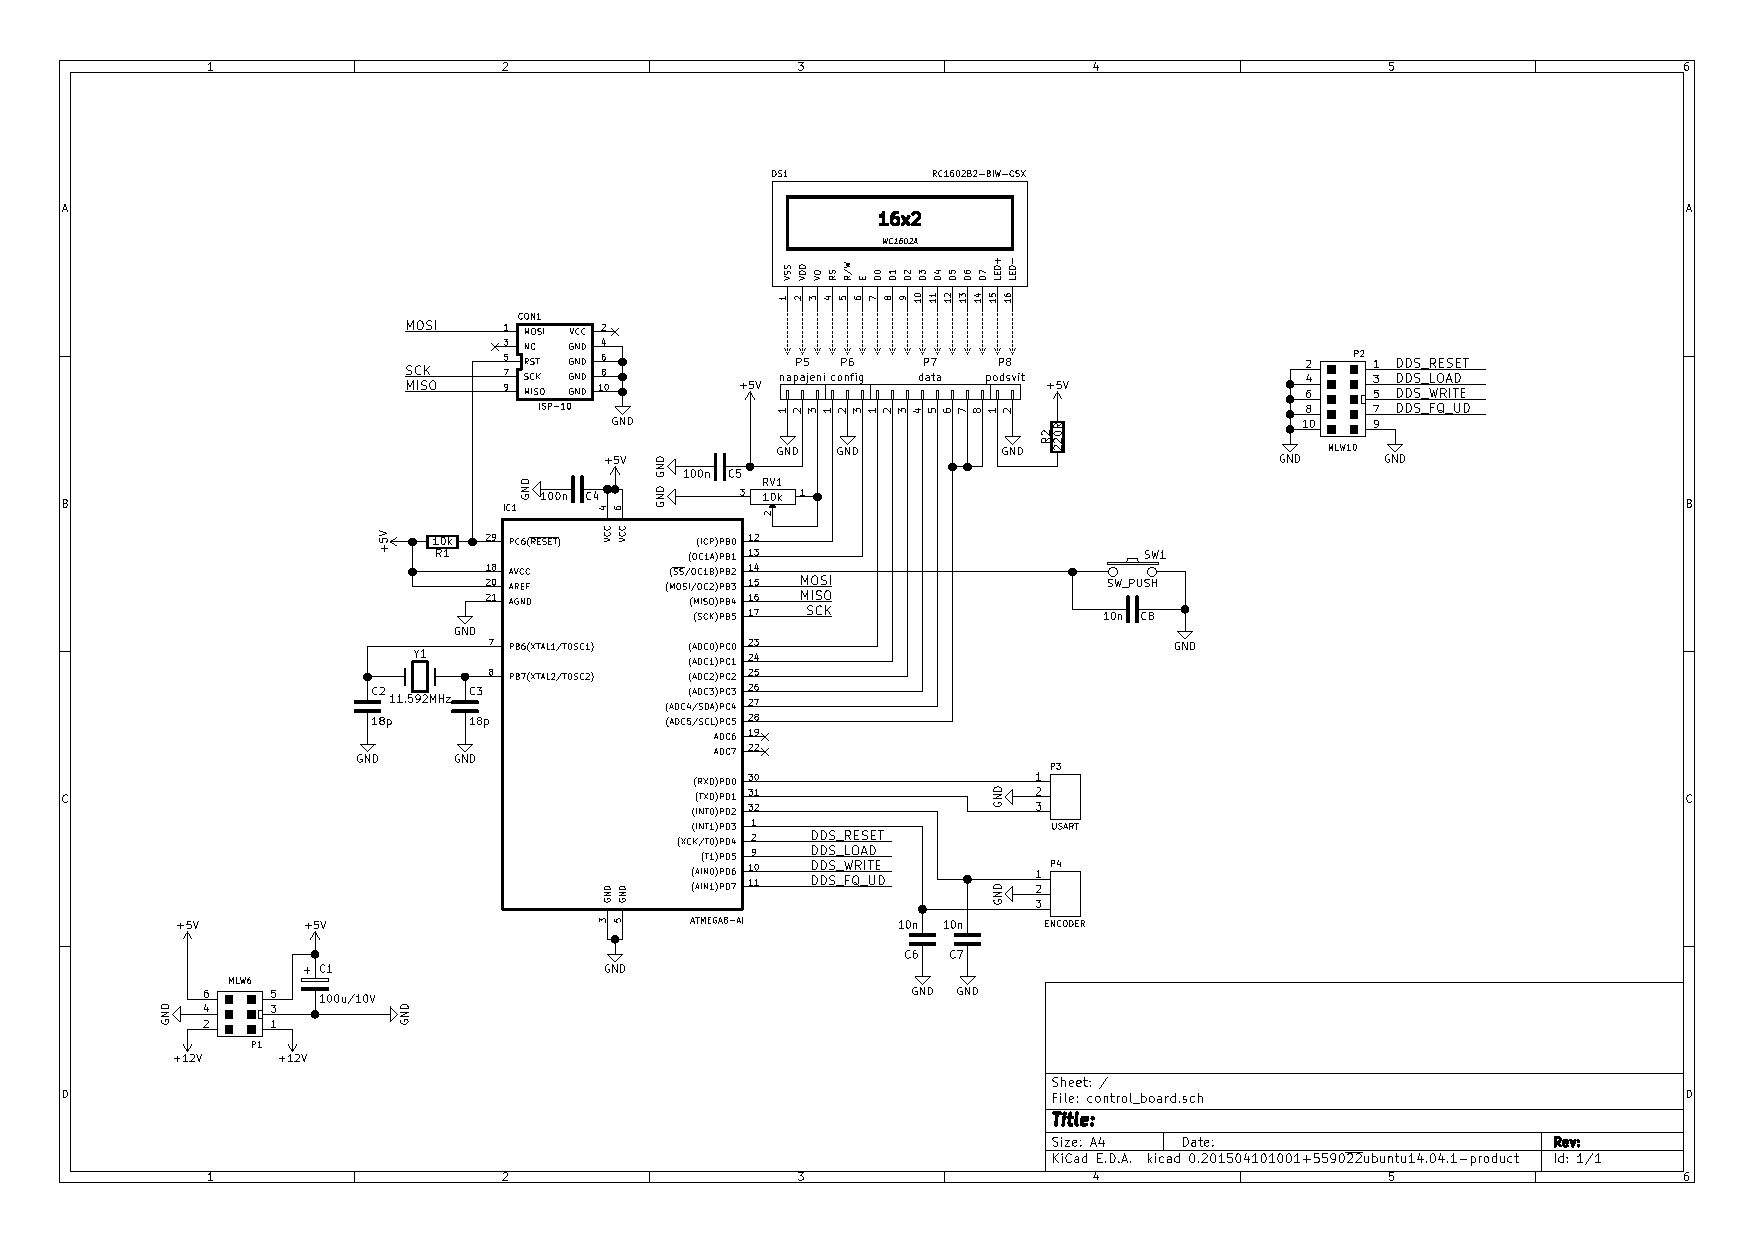
\includepdf[landscape=true]{img/cu/sch.pdf}

% DPS
\begin{figure}[H]
	\centering
	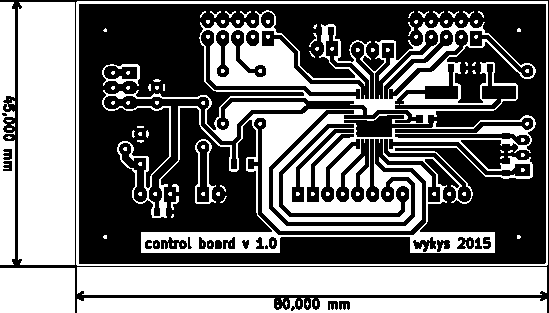
\includegraphics[width=170mm]{img/cu/cu_b.pdf}
	\caption{Deska plošného spoje řídící jednotky, strana spojů}    		
\end{figure}

% os f
\begin{figure}[H]
	\centering
	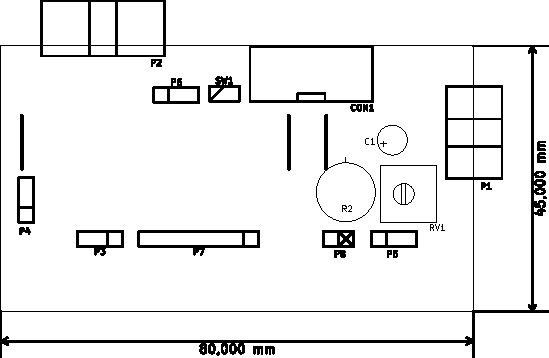
\includegraphics[width=170mm]{img/cu/os_f.pdf}
	\caption{Osazovací plán řídící jednotky, strana součástek}    		
\end{figure}

% os b
\begin{figure}[H]
	\centering
	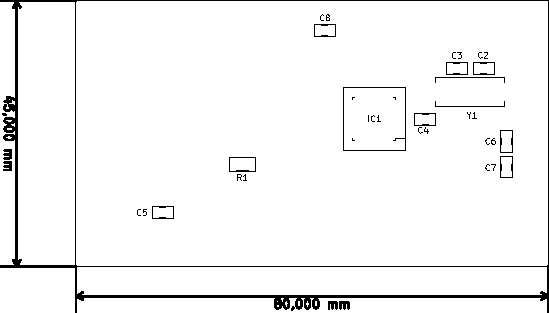
\includegraphics[width=165mm]{img/cu/os_b.pdf}
	\caption{Osazovací plán řídící jednotky, strana spojů}    		
\end{figure}

\begin{table}[H]
	\begin{center}
		\caption{Tabulka použitých součástek pro desku řídící jednotky}
		\label{tab:cu_os}      
		\begin{tabular}[H]{!{\vrule width 1pt}c|c|c|c!{\vrule width 1pt}}
		    \specialrule{1pt}{0pt}{0pt} 
		    \textbf{Určovatel}	&	\textbf{Pouzdro}	&	\textbf{Množství}	&	\textbf{Určení}	\\\specialrule{1pt}{0pt}{0pt} 
			C1	&	Elko\_vert\_11x5mm\_RM2.5\_CopperClear	&	1	&	100u/10V	\\\hline
			C2,C3	&	C\_0805	&	2	&	18p	\\\hline
			C4,C5	&	C\_0805	&	2	&	100n	\\\hline
			C6,C7,C8	&	C\_0805	&	3	&	10n	\\\hline
			CON1	&	vasch\_strip\_5x2	&	1	&	ISP-10	\\\hline
			IC1	&	TQFP-32\_7x7mm\_Pitch0.8mm	&	1	&	ATMEGA8-AI	\\\hline
			P1	&	vasch\_strip\_3x2\_90	&	1	&	MLW6	\\\hline
			P2	&	vasch\_strip\_5x2\_90	&	1	&	MLW10	\\\hline
			R1	&	R\_1206	&	1	&	10k	\\\hline
			RV1	&	Potentiometer\_Trimmer-Suntan-TSR-3386P	&	1	&	10k	\\\hline
			Y1	&	Crystal\_HC49-SD\_SMD	&	1	&	11.592MHz	\\\hline
			P5	&	pin\_socket\_3	&	1	&	napajeni	\\\hline
			P6	&	pin\_socket\_3	&	1	&	config	\\\hline
			P7	&	pin\_socket\_8	&	1	&	data	\\\hline
			P8	&	pin\_socket\_2	&	1	&	podsvit	\\\hline
			P4	&	pin\_strip\_3	&	1	&	ENCODER	\\\hline
			P3	&	pin\_strip\_3	&	1	&	USART	\\\hline
			SW1	&	pin\_strip\_2	&	1	&	SW\_PUSH	\\\hline
			R2	&	Resistor\_Vertical\_RM7.5mm	&	1	&	220R	\\\hline
			M1,M2,M3,M4	&	M3	&	4	&	M3	\\\specialrule{1pt}{0pt}{0pt} 
		\end{tabular}
	\end{center}
\end{table}

